\section{KORD Temperature Prediction Using Selected Airport Features}
This analysis implements multivariate time series regression models to predict temperature at Chicago O'Hare International Airport (KORD) using weather data from selected airports. The model incorporates both historical data and recent changes in weather patterns across these airports.\n\begin{itemize}
  \item Base Model: Multivariate Linear Regression
  \item Feature Engineering: Airport-specific features with time lags and 2-hour changes
  \item Prediction Horizons: Multiple time windows (1h, 24h, 5d, 5d avg, 30d avg)
  \item Train/Test Split: 80/20
  \item Random State: 42 (for reproducibility)
  \item Validation: Standard train-test split
\end{itemize}

\subsection{1 Hour Ahead Temperature Prediction for KORD}
\subsection{Model Performance}
\begin{tabular}{llr}
\toprule
 & Metric & Value \\
\midrule
0 & Root Mean Squared Error (RMSE) & 1.11 \\
1 & Mean Absolute Error (MAE) & 0.82 \\
2 & R^2 Score & 0.99 \\
\bottomrule
\end{tabular}

\subsection{1 Hour Ahead Predictions}
\begin{figure}[htbp]
\centering
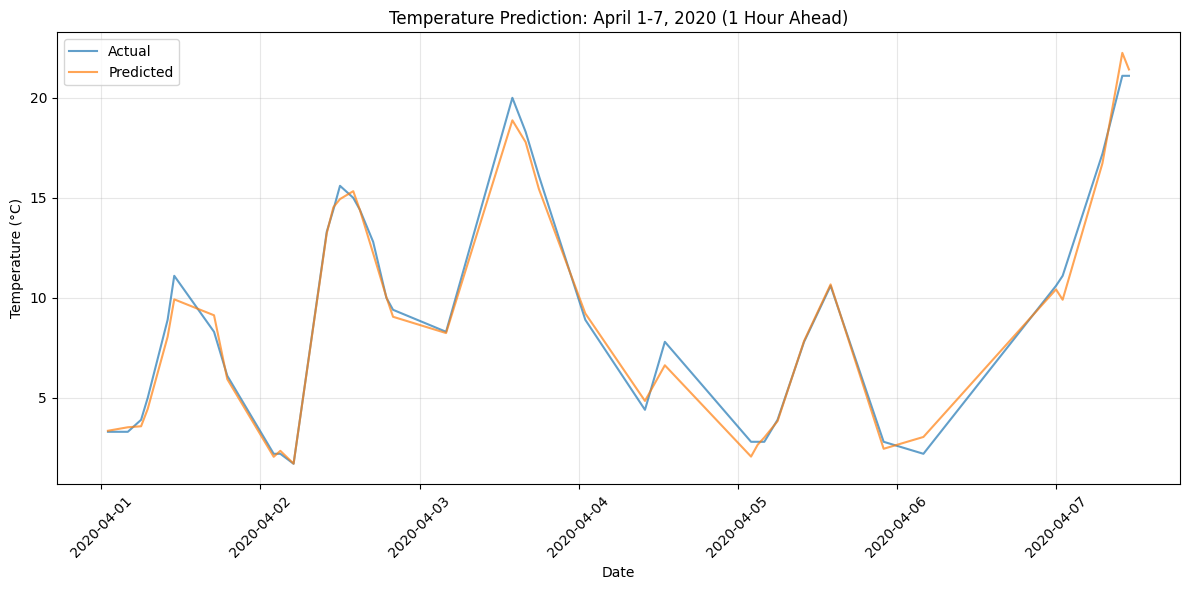
\includegraphics[width=0.7\textwidth]{1-0-linear_temp_shift_results.png}
\caption{1 Hour Ahead Predictions for KORD}
\label{fig:1_hour_ahead_pred}
\end{figure}

\subsection{1 Hour Ahead Feature Importance}
\begin{figure}[htbp]
\centering
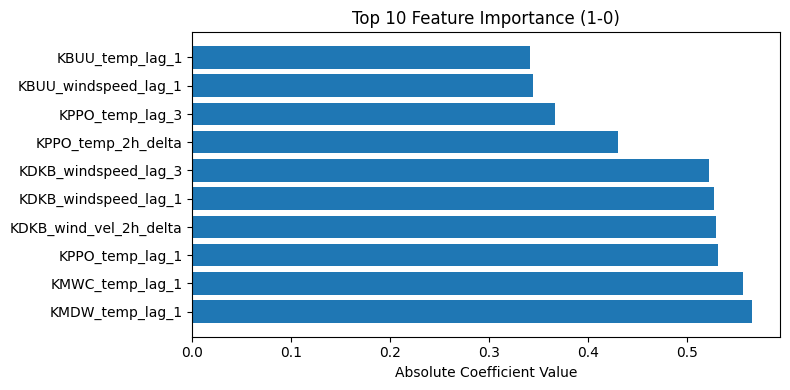
\includegraphics[width=0.7\textwidth]{1-0-linear_temp_shift_feature_importance.png}
\caption{1 Hour Ahead Feature Importance}
\label{fig:1_hour_ahead_featimp}
\end{figure}



\subsection{24 Hours Ahead Temperature Prediction for KORD}
\subsection{Model Performance}
\begin{tabular}{llr}
\toprule
 & Metric & Value \\
\midrule
0 & Root Mean Squared Error (RMSE) & 3.93 \\
1 & Mean Absolute Error (MAE) & 3.01 \\
2 & R^2 Score & 0.88 \\
\bottomrule
\end{tabular}

\subsection{24 Hours Ahead Predictions}
\begin{figure}[htbp]
\centering
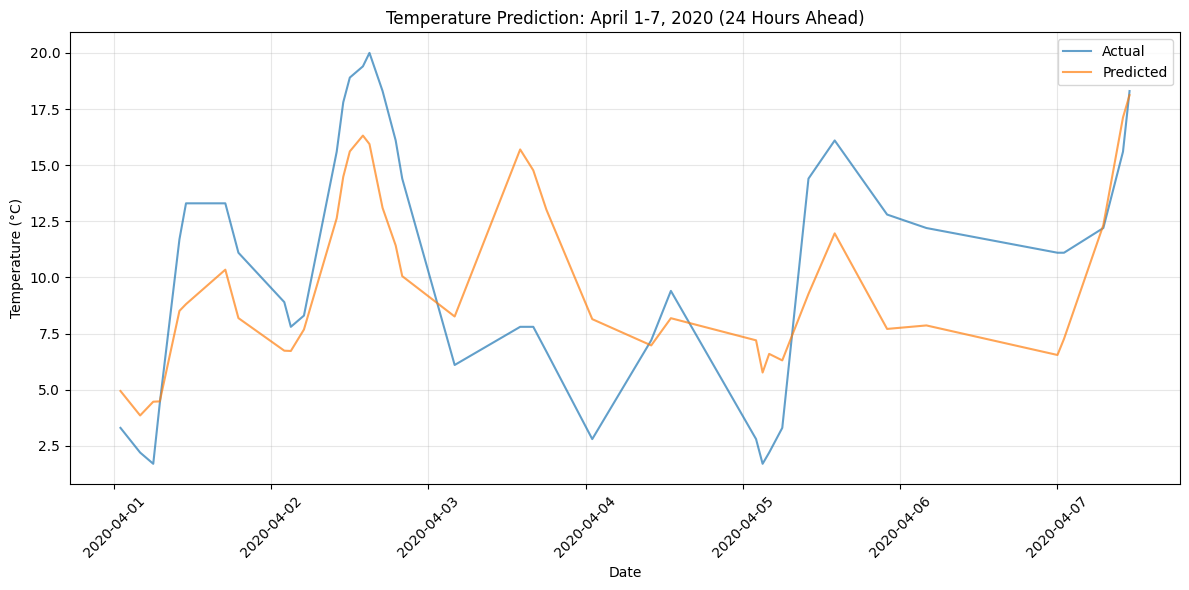
\includegraphics[width=0.7\textwidth]{1-1-linear_temp_shift_results.png}
\caption{24 Hours Ahead Predictions for KORD}
\label{fig:24_hours_ahead_pred}
\end{figure}

\subsection{24 Hours Ahead Feature Importance}
\begin{figure}[htbp]
\centering
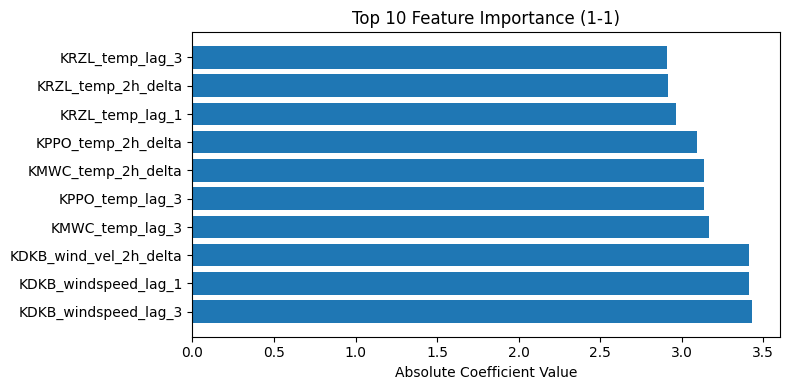
\includegraphics[width=0.7\textwidth]{1-1-linear_temp_shift_feature_importance.png}
\caption{24 Hours Ahead Feature Importance}
\label{fig:24_hours_ahead_featimp}
\end{figure}



\subsection{120 Hours (5 Days) Ahead Temperature Prediction for KORD}
\subsection{Model Performance}
\begin{tabular}{llr}
\toprule
 & Metric & Value \\
\midrule
0 & Root Mean Squared Error (RMSE) & 5.64 \\
1 & Mean Absolute Error (MAE) & 4.41 \\
2 & R^2 Score & 0.75 \\
\bottomrule
\end{tabular}

\subsection{120 Hours (5 Days) Ahead Predictions}
\begin{figure}[htbp]
\centering
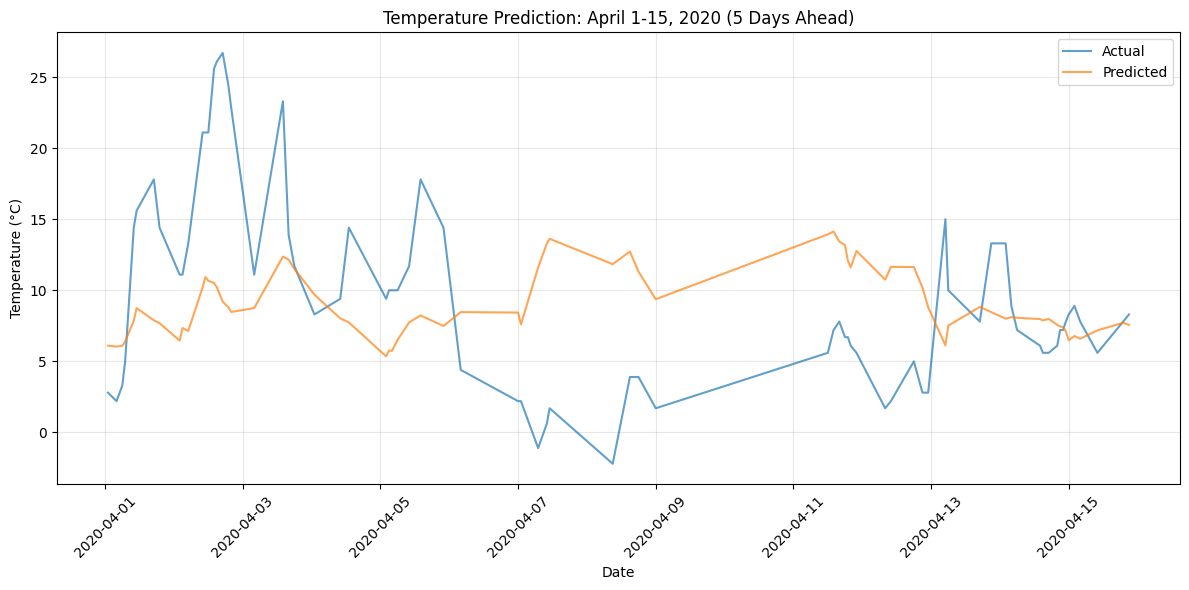
\includegraphics[width=0.7\textwidth]{1-2-linear_temp_shift_results.png}
\caption{120 Hours (5 Days) Ahead Predictions for KORD}
\label{fig:120_hours_(5_days)_ahead_pred}
\end{figure}

\subsection{120 Hours (5 Days) Ahead Feature Importance}
\begin{figure}[htbp]
\centering
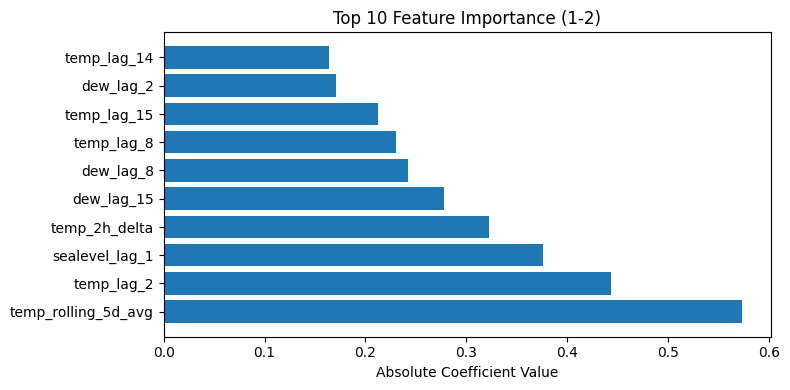
\includegraphics[width=0.7\textwidth]{1-2-linear_temp_shift_feature_importance.png}
\caption{120 Hours (5 Days) Ahead Feature Importance}
\label{fig:120_hours_(5_days)_ahead_featimp}
\end{figure}



\subsection{5-Day Average Ahead Temperature Prediction for KORD}
\subsection{Model Performance}
\begin{tabular}{llr}
\toprule
 & Metric & Value \\
\midrule
0 & Root Mean Squared Error (RMSE) & 3.30 \\
1 & Mean Absolute Error (MAE) & 2.58 \\
2 & R^2 Score & 0.90 \\
\bottomrule
\end{tabular}

\subsection{5-Day Average Ahead Predictions}
\begin{figure}[htbp]
\centering
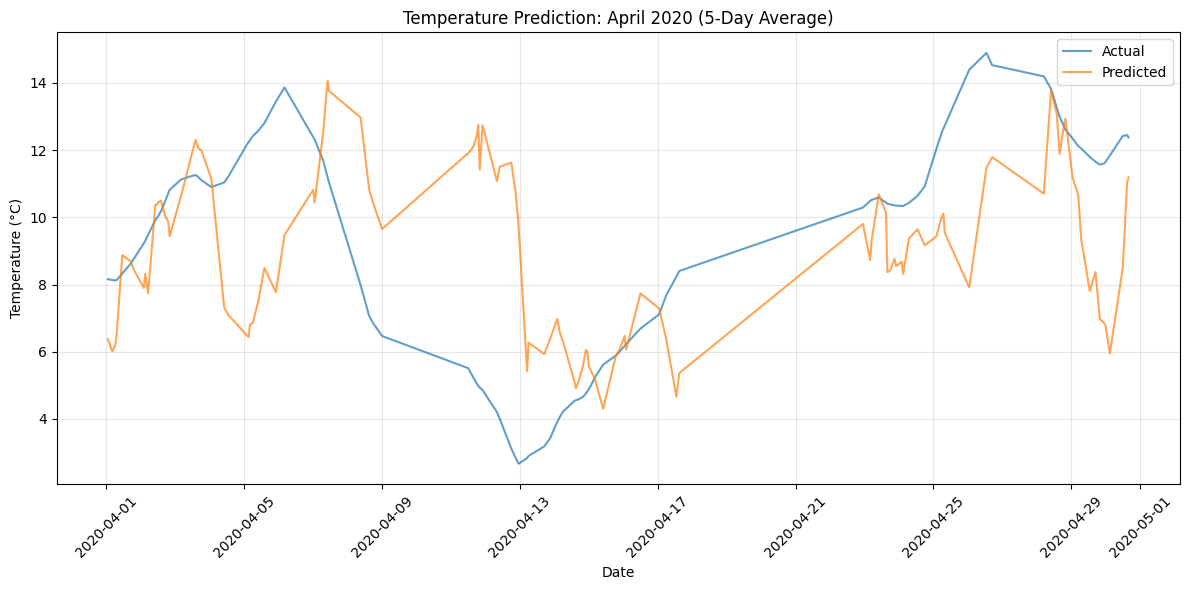
\includegraphics[width=0.7\textwidth]{1-3-linear_temp_shift_results.png}
\caption{5-Day Average Ahead Predictions for KORD}
\label{fig:5-day_average_ahead_pred}
\end{figure}

\subsection{5-Day Average Ahead Feature Importance}
\begin{figure}[htbp]
\centering
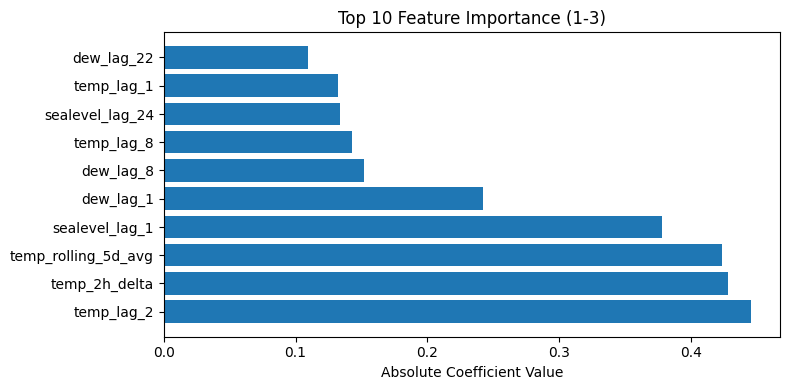
\includegraphics[width=0.7\textwidth]{1-3-linear_temp_shift_feature_importance.png}
\caption{5-Day Average Ahead Feature Importance}
\label{fig:5-day_average_ahead_featimp}
\end{figure}



\subsection{30-Day Average Ahead Temperature Prediction for KORD}
\subsection{Model Performance}
\begin{tabular}{llr}
\toprule
 & Metric & Value \\
\midrule
0 & Root Mean Squared Error (RMSE) & 3.55 \\
1 & Mean Absolute Error (MAE) & 2.84 \\
2 & R^2 Score & 0.87 \\
\bottomrule
\end{tabular}

\subsection{30-Day Average Ahead Predictions}
\begin{figure}[htbp]
\centering
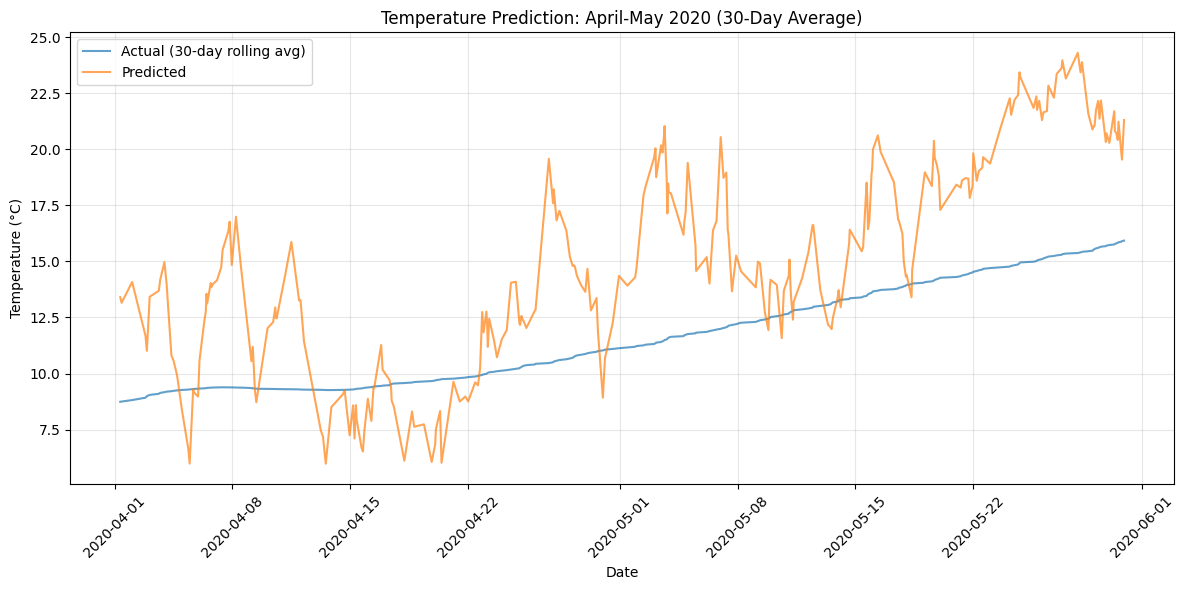
\includegraphics[width=0.7\textwidth]{1-4-linear_temp_shift_results.png}
\caption{30-Day Average Ahead Predictions for KORD}
\label{fig:30-day_average_ahead_pred}
\end{figure}

\subsection{30-Day Average Ahead Feature Importance}
\begin{figure}[htbp]
\centering
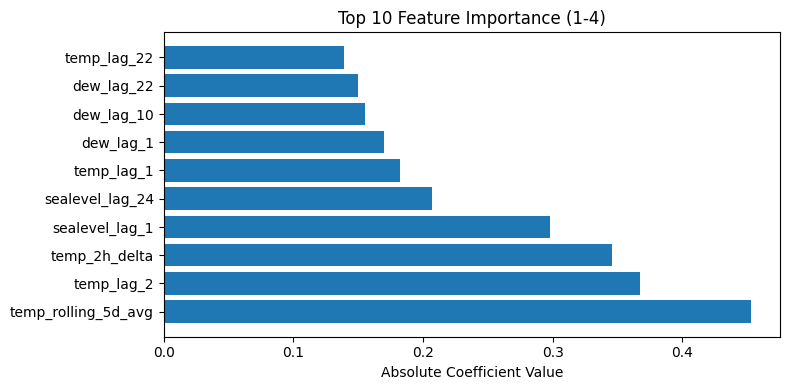
\includegraphics[width=0.7\textwidth]{1-4-linear_temp_shift_feature_importance.png}
\caption{30-Day Average Ahead Feature Importance}
\label{fig:30-day_average_ahead_featimp}
\end{figure}


\section{Model Interpretation}

These multivariate regression models capture the complex relationships between weather patterns across multiple airports and temperature at KORD. The models:\
egin{itemize}
  \item Use weather conditions from selected airports to predict KORD's temperature
  \item Account for recent changes in weather patterns through 2-hour delta features
  \item Incorporate historical weather patterns through lagged features
  \item Help identify which airports' weather patterns most influence KORD's temperature
\end{itemize}
Future improvements could include:\
egin{itemize}
  \item Feature selection to reduce dimensionality
  \item Non-linear models to capture complex relationships
  \item Time series specific models (ARIMA, LSTM)
  \item Spatial relationship modeling between airports
\end{itemize}

